\documentclass[12pt]{article}

\textwidth=6.5in
\textheight=8.5in
\topmargin=0in
\headheight=0.5in
\headsep=0in
\footskip=0.25in
\oddsidemargin=0in
%\pagestyle{headings}
\usepackage{listings}
\usepackage{graphicx}
\usepackage{parskip}
\usepackage{amsmath}
\usepackage{hyperref}


\begin{document}

\begin{centering}
\section*{The Transmission Line}
\end{centering}

Update: Matt 21Mar2026 (\today)
\tableofcontents

\section{Introduction}




This lab involves a good dose of electronics and electromagnetics.  Dust off your PHYS-143 and PHYS-206 knowledge for this one.

A transmission line is two conductors that do not touch for the entire length of the line. The two conductors can be thought of as a \emph{signal} and \emph{return}.  Transmission lines are used to transmit signals in the form of electromagnetic energy over some needed distance, for example, between one device and another.  The black cables in your house for cable-television or ethernet cables for data are examples of transmissions lines.

A coaxial transmission line has its two conductors sharing a common axis of cylindrical symmetry that runs the length of the cable. There is a small diameter inner conductor which resembles a long bare copper wire.  This is wrapped in an insulating dielectric, then surrounded by an outer conducting sheath.  The entire assembly is then wrapped in a rubber or plastic coating for protection. An example is shown here (from Wikipedia).


\begin{figure}[h]
\centering 
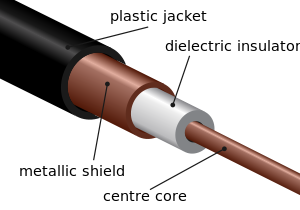
\includegraphics[scale=0.5]{Figs/coax.png}
\end{figure}

In this lab, we'll study some electrical properties of coaxial cables, then look at how signals propagate through them.

\subsection{Resistance, Capacitance, Inductance, and AC vs. DC}

Note that a transmission line, despite just being two separated conductors, is quite complicated from an electrical standpoint. This is what we'll study in this lab. 

As we begin, note that the three properties all electrical devices have are resistance, capacitance, and inductance.  In your introductory physics course, you studied all of these from a DC standpoint. Here, DC means a constant voltage.  Resistance $(R)$ led to Ohms law, $V=IR$, capacitance $(C)$ led to the ability to separate and hold charge $Q=CV$, and inductance $(L)$ is the proportionality constant between magnetic flux and current, or $\Phi_B=LI$.

It is rare for DC voltages to be used with transmission lines. Usually AC voltages are used, as we will do in this lab. Think: sine waves or pulses. This means the frequency of the AC voltage will be a critical parameter.  From an electrical standpoint, resistors behave essentially the same under AC as they do in DC. 

Capacitors and inductors however, behave differently due to AC stimulation.  Capacitors present a reactance to AC called ``capacitive reactance'' which is $X_C=1/(2\pi fC)$.  Inductors present an ``inductive reactance'' of $X_L=2\pi fL$. Both have units of Ohms, and note that unlike the familiar constant $R$, the reactance of a capacitor and inductor depends on the applied frequency, $f$. Reactances do not have linear, ohmic behavior that follow Ohm's law like a resistor does.

Lastly, as we said, all electrical devices have resistance, capacitance, and inductance. They work together to present a ``total resistance'' to an AC signal. This effective resistance is termed ``impedance,'' and is given the symbol $Z$.  All told, the impedance of a device is

\begin{equation}
\label{Z}
Z=\sqrt{R^2+(X_C-X_L)^2},
\end{equation}

which is the total Ohms an AC signal will experience when applied to a device, such as a transmission line.  Note again, $R$ is constant here, but $X_C$ and $X_L$ depend on frequency, so $Z$ will also depend on frequency. That's right: electrical devices have a frequency-dependent resistance. This is an important theme in this lab.



 
\section{Theory}

This section includes some derivations. Treat all derivations like ``data'' you took, meaning fully include and present them in your report.

\subsection{Derivations}

To begin, derive from first principles, the capacitance per unit length (${\tilde C}$) and inductance per unit length (${\tilde L}$) of a coaxial arrangement of conductors. These are PHYS-143 level problems. You can find help in any book for that level of class. Hints:

\begin{enumerate}

\item For the capacitance per unit length, you can find help by looking up a ``cylindrical capacitor.'' This will involve Gauss's law, $\Delta V=-\int {\vec E}\cdot d{\vec l}$, and the definition of capacitance, $C=Q/V$. (See Example 2, p. 746 of \url{https://b-ok.cc/book/5329620/fc9583}).

\item For the inductance per unit length, you'll need Ampere's Law,  $\Phi_B=\iint {\vec B}\cdot d{\vec A}$, and the definition of inductance, $\Phi_B=LI$. You can find help by paralleling the derivation for a rectangular toroid (the coaxial transmission line is a toroid that is all stretched out and circular, not rectangular). (See Example 1 on p. 901 of \url{https://b-ok.cc/book/5329620/fc9583}).

\end{enumerate}

Include your derivations, this should involve a figure of each system (Gaussian surface, integral paths, etc.) helping the derivation along.

\subsection{Calculations}

Measure the diameter of the inner and outer conductors, and compute numerical values for  ${\tilde C}$ and  ${\tilde L}$.  Also, find out the total length of the transmission line.  Hang on to these values and formulas. They'll come up again. For now, are you sure of your choices for values of $\mu_0$ and $\epsilon_0$?

\section{Capacitive and Inductive Measurements}

\subsection{Voltage divider}

Review a two-resistor voltage divider from PHYS-206. The Wikipedia page \url{https://en.wikipedia.org/wiki/Voltage_divider} is ideal. Have the structure and equation for $V_\text{out}$ as a function of $V_\text{in}$, $Z_1$ and $Z_2$ handy. Assume $Z_1$ is connected to $+V_\text{in}$ and $Z_2$ is connected to ground. Note: In PHYS-206, the voltage divider equation was originally written with $R$'s instead of $Z$'s. The $Z$'s are used when considering resistance of AC signals and are called ``impedance'' instead of resistance.  All have units of Ohms.

\subsubsection{Capacitance of the transmission line}

The two conductors of a transmission line behave like a {\sl capacitor} if the far end of the transmission line is open circuited.  Explain why in your report.

Build a voltage divider using a $10$ k$\Omega$ resistor as $Z_1$ and $Z_2$ as the transmission line itself.

Note here, $Z_1=10,000\ \Omega$ and $Z_2=X_c$ where $X_c$ is the capacitive reactance of the transmission line, which is $X_c=1/(2\pi fC)$. Plug these values/quantities into the equation for a voltage divider and solve for $C$. 

To prepare for data analysis, linearize your equation for $C$, so the slope of a linear fit can be used to find $C$. (See the PDF in this repo.)

Next, place an AC signal across the voltage divider. Monitor the peak-to-peak voltage on CH1 of your oscilloscope, which is $V_\text{in}$. On CH2, monitor the peak to peak voltage across the transmission line, which is $V_\text{out}$. Measure $V_\text{out}$ vs. $V_\text{in}$ for a variety of driving frequencies from 1000 - 10,000 Hz. Use this data and your linearized equation for $C$ to perform a curve fit. Use your fit parameters to find $C$. This is the capacitance of the transmission line.


You now have a measured $C$ and a theoretical ${\tilde C}$ from your derivation. Compare the two noting that $C$ is capacitance and ${\tilde C}$ is capacitance \emph{per unit length}.

\subsection{The RLC Circuit}

An LC circuit consists of an inductor ($L$) and capacitor ($C$) as shown here.

\begin{figure}[h]
\centering 
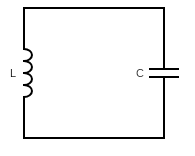
\includegraphics[scale=1]{Figs/LC.png}
\label{lc_circuit}
\end{figure}

Using Kirchoff's Law for the loop, $\Sigma V=0$ (around the loop), set up and solve a differential equation that will lead to a formula for the fundamental frequency of such a circuit. Recall for an inductor that $\Delta V_L=-LdI/dt$ and for a capacitor $\Delta V_C=Q/C$.  You should get a fundamental frequency of $\omega_{LC}=1/\sqrt{LC}$. Note also that $\omega$ is in rad/s, convenient for math, but lab equipment measures $f$ in Hz, which is $f=\omega/2\pi$.

\subsubsection{Inductance of the transmission line}

The two conductors of a transmission line are an inductor if the far end of the transmission line is short circuited.  Explain why in your report.

Build an LC circuit using a capacitor and the transmission line as the $L$. {\bf decade box?} Here three different capacitors will be used, a $269$ nF, $1\ \mu$F, and a $10\ \mu$F.  Put a $50\  \Omega$ resistor in series with them.  Apply an AC voltage across the whole circuit. Monitor this voltage on CH1 and the voltage across just the resistor on CH2.

You should go off now and search for the resonance frequency of this circuit. Once found, you can use your result for the resonance frequency of an $LC$ circuit (above) to find $L$, the inductance of the transmission line.  

How does one find the resonance frequency?  With the circuit connected, explore frequencies between 100 and 50,000 Hz. Steps of 1,000 Hz should suffice.  When resonance is hit, the impedance of the capacitor and inductor will become equal. Reviewing Eq.~\ref{Z}, this means $Z=R$, or the LRC circuit will show its smallest impedance (i.e. $Z=\sqrt{R^2+0})$ and be purely ohmic in behavior.  This will maximize the current that flows through the resistor ($I=V/Z$, with $Z\rightarrow$ small), and hence the voltage drop across it. This means as you explore, the resonance frequency will cause a maximum of the AC amplitude on CH2.

To analyze this data, plot the CH2 voltage vs frequency.  Since you explored a couple of orders of magnitude in frequency, plot the log (base 10) of frequencies on the horizontal axis, and voltage on the vertical axis. It should appear like a peaked function that is very wide.  The center of this peak is the resonance frequency. Do a curve fit to find it. It is not clear what function to use. Consider {\sl some function} that is peaked and has a center as a parameter.

Repeat for two more capacitors. Here $1\ \mu$F and $10\ \mu$F capacitors were used in addition to the $269$ nF. When done, you should have 3 resonant frequencies, one for each capacitor value.  Find a linearized form of $f=1/(2\pi\sqrt{LC})$. Do a linear curve fit of your data and find $L$ from the slope.

\subsubsection{Corrections to L}

Compare the $L$ you measured with ${\tilde L}$ from above, noting that $L$ is inductance and ${\tilde L}$ is inductance per unit length. They generally won't match. Why? 

The hard boundary for the diameter of the inner conductor assumes a high frequency AC signal. Higher frequency currents tend to travel on the surface of conductors, which may very well be at the diameter you measured.  But lower frequencies will travel at more depths within the conductor.  The ``skin depth'' parameter is a measure of this depth, which is

\begin{equation}
\delta=\sqrt{\frac{2\rho}{\omega \mu_0}},
\end{equation}

where $\rho$ is the resistivity of the conductor, $\omega$ is the angular frequency of the AC signal, and $\mu_0$ is the usual constant. Evaluate this for some central frequency you used in your inductor measurements. Does your result warrant a correction to the diameter of the inner conductor used to compute ${\tilde L}$? If so, by how much, and can this bring ${\tilde L}$ into better agreement with the $L$ you measured?

\subsection{Meter}

Use the $L$, $R$, or $C$ meter to directly measure the $L$, $R$, and $C$ of the transmission line.  Use these numbers for comparison with those above. 

\subsection{Stop and check}

At this point, you should have several numbers associated with the coaxial transmission line dealing with capacitance and inductance, including experimental, theoretical, and those from the meter. There will be varying degrees of agreement between them all. The skin depth consideration provides some range that your theoretical $L$ and $C$ can be.

Uses of these numbers and some reconciliation of them all will be forthcoming in the following sections.

\section{Pulse Propagation}

As mentioned, transmission lines are used to send signals between devices.  Let's look at this further. What we'll do is to send a digital binary 1 down the coaxial transmission line. This binary 1 will be in the form of a single voltage pulse.

Before continuing, go to \url{https://phet.colorado.edu/en/simulation/wave-on-a-string} and run the simulation. Select: Pulse, 1.25 cm amplitude, 0.65 s width, no damping, and low tension. This pulse will be the binary 1 you are sending down the line. Explore what happens to the initial rightward moving pulse with:

\begin{enumerate}
\item Both fixed and loose ends to the transmission line.
\item If there's no end to the transmission line (i.e. infinitely long).
\end{enumerate}

Suppose the rope was 1000 ft long and you only had access to the launch end of it (the other end is too far away).  Do you think it would be possible to determine how fast the pulse travels in the rope with such access to just the launch end? Explain how.

\subsection{Pulse Speed in transmission line}

Connect the pulse generator to both the oscilloscope and the transmission line.  Be sure the far end of the transmission line is open-circuited.   Choose a maximum amplitude and a pulse width of about $10$ ns. In addition to the obvious launch pulse, there should be another interesting feature on the oscilloscope display.  Think of the simulation now: what is the origin of this feature, and can you use it compute the pulse's propagation speed in the transmission line (use your same logic as in the simulation above)? (Note: Think carefully about the total distance travelled by the pulse.)

So you now have the speed at which information travels in a transmission line. How does it compare with the speed of light?

\subsubsection{Pulse speed propagation: theory}

As you may know, the pulse is a superposition of electromagnetic waves. Why? How does one make a pulse? Go to this page \url{https://phet.colorado.edu/en/simulation/legacy/fourier}, select ``wave-packet'' (the closest thing to a pulse), and look at all of {\sl the waves} in the center graph needed to make a pulse.

The time dependent position of the pulse down the transmission line necessarily means that it has a time varying electric field (or $E$-field). Any time varying $E$-field also gives rise to a time varying $B$-field (and vise versa); this is Faraday's Law.  Supposing the $E$-field is traveling wave, or $E=E_0\sin(kx-\omega t)$ and the $B$-field is  $B=B_0\sin(kx-\omega t)$, they are related by

\begin{equation}
-\frac{\partial B}{\partial x}=\mu_0 \epsilon_0 \frac{\partial E}{\partial t}.
\end{equation}

Note the usual definitions of $k=2\pi/\lambda$ and $\omega=2\pi f$.  Plug the functions for $E$ and $B$ into this, and note that for $E_0$ and $B_0$ (in an electromagnetic wave), $E_0=vB_0$, where $v$ is the speed of the wave (in this case, an electromagnetic wave). Compute a theoretical value for the speed of the wave.  (Note in physics that $\mu_0=4\pi\times 10^{-7}$ m/A (exactly) and $\epsilon_0$ is experimentally determined.)

Notice anything? What does your $v$ come out to be? (This derivation of the speed of light in terms of the two fundamental constants is a huge success of Maxwell's equations and is a classic one. All physics majors should know this.)

\subsection{Pulse speed propagation: transmission line}

The derivation for $c$ above was assumed to be in free space.  The pulse in the transmission line is in the copper conductor, and has that dielectric between the two conductors. This is not free space.  You should also have noted how the pulse speed $v_\text{pulse}<c$. This is useful to know. Why? Well, you may know from optics that the speed of light in some material with an index of refraction $n$ (like glass) is less that $c$ too, in fact $v=c/n$.\footnote{It's really not less, we just tell that to introductory physics students.} 

For an electromagnetic pulse that is not in free space, $v=1/\sqrt{\mu\epsilon}$ (similar to your derivation), where $\mu=\chi\mu_0$ and $\epsilon=\kappa \epsilon_0$. Here $\chi$ is the magnetic sucseptibility and $\kappa$ is the dielectric constant.  For the transmission line $\chi\approx 1$, and you can use your pulse propagation speed to reconcile some of your numbers. In particular:

\begin{enumerate}
\item Compute $\kappa$ from the relations above $(v=1/\sqrt{\chi\mu_0\kappa\epsilon_0})$.
\item The capacitance of a capacitor is increased by the presence of a dielectric, namely $C_\text{with-dielectic}=\kappa C_\text{without-dielectric}$.  So you can now scale your theoretical value of $C$ (derived with no dielectric assumed) of your transmission line to what you determined experimentally and or from the meter.
\end{enumerate}

\section{Impedance of the transmission line}
                             
As you can tell by now, the inductance and capacitance of a transmission line play a huge role in how it behaves electrically. We've seen inductive resonances, capacitive voltage division, and propagation speed reductions (relative to $c$) due to the dielectric.  

In the introduction, we said that all electrical devices have resistance, capacitance, and inductance. They work together to present a ``total resistance'' to an AC signal, which is called $Z$, the ``impedance'' of the device. Let's see if we can arrive at the impedance of the transmission line.

\subsection{Transmission line impedance: a model}

\subsubsection{Circuit analysis review and warm-up}

To begin, let's review a bit of introductory physics and circuit analysis. Consider the circuit in Fig.~\ref{z01}.

\begin{figure}[h]
\centering 
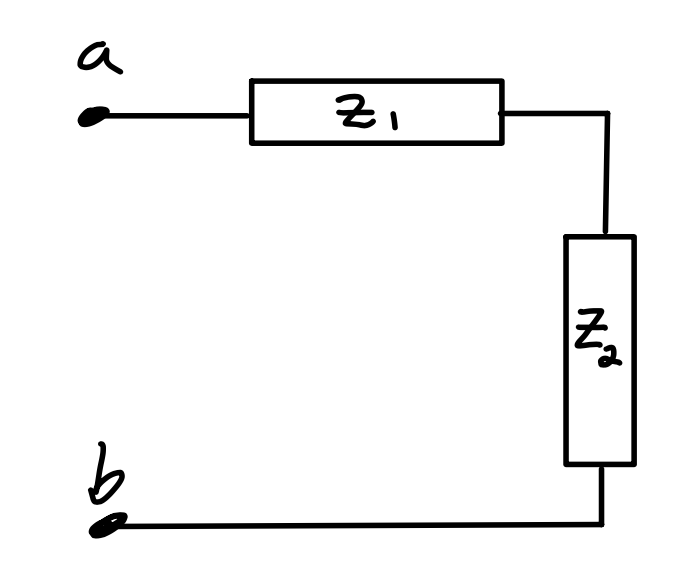
\includegraphics[scale=0.5]{Figs/Feynman/z01.png}
\caption{A series circuit.}
\label{z01}
\end{figure}

Here $Z_1$ and $Z_2$ are impedances of two circuit elements in series. What is the net impedance between points $a$ and $b$?  For elements in series $Z_3=Z_1+Z_2$, so the whole circuit can be represented by the single element $Z_3$ as shown in Fig.~\ref{z02}.

\begin{figure}[h]
\centering 
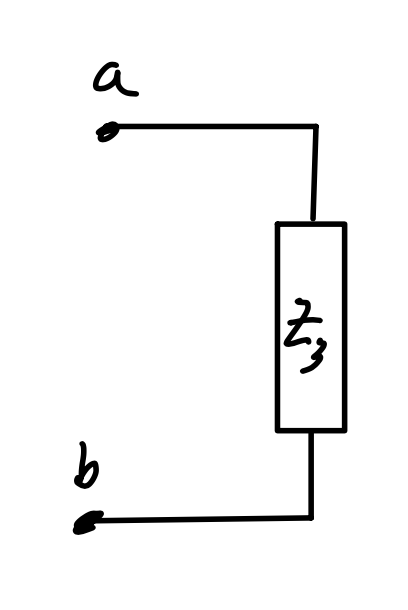
\includegraphics[scale=0.5]{Figs/Feynman/z02.png}
\caption{A equivalent circuit to that in Fig.~\ref{z01}.}
\label{z02}
\end{figure}

A more complicated circuit would be something like Fig.~\ref{z03}. 

\begin{figure}[h]
\centering 
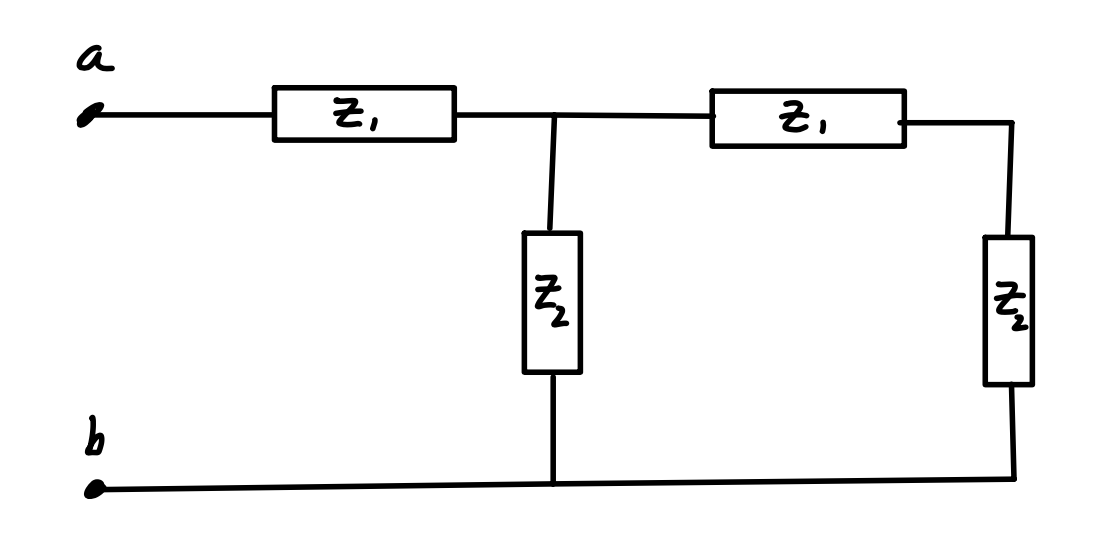
\includegraphics[scale=0.5]{Figs/Feynman/z03.png}
\caption{A more complicated but still reducible circuit.}
\label{z03}
\end{figure}

Here we start by putting $Z_3=Z_1+Z_2$ (since they're in series), and arrive at Fig.~\ref{z04}.  Then, we see that $Z_2$ and $Z_3$ are in parallel, so we could reduce this to Fig.~\ref{z05} with $Z_4=1/(1/Z_2+1/Z_3)$ and finally to Fig.~\ref{z06}, with $Z_5=Z_1+Z_4$. So the impedance across $a$ and $b$, in Fig~\ref{z06}, is the same as that in the original circuit.

\begin{figure}[h]
\centering 
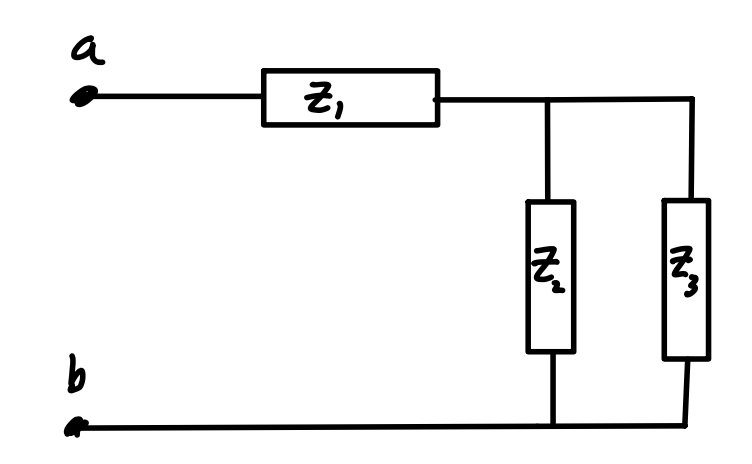
\includegraphics[scale=0.5]{Figs/Feynman/z04.png}
\caption{A step in reducing the circuit in Fig.~\ref{z03}.}
\label{z04}
\end{figure}



\begin{figure}[h]
\centering 
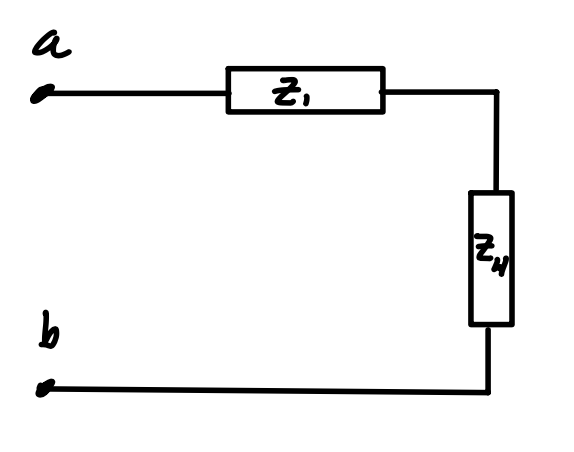
\includegraphics[scale=0.5]{Figs/Feynman/z05.png}
\caption{A step in reducing the circuit in Fig.~\ref{z04}.}
\label{z05}
\end{figure}

\begin{figure}[h]
\centering 
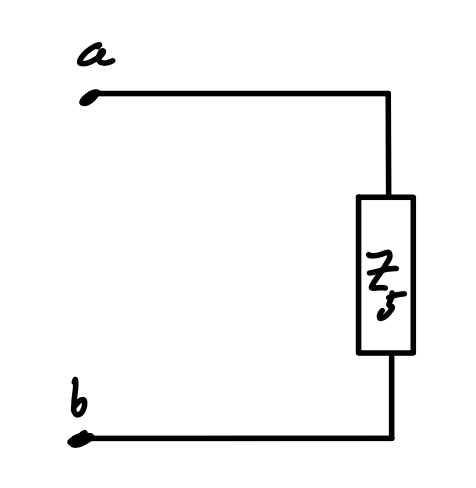
\includegraphics[scale=0.5]{Figs/Feynman/z06.png}
\caption{A step in reducing the circuit in Fig.~\ref{z05}.}
\label{z06}
\end{figure}

\subsubsection{Model a transmission line}

With that circuit analysis review done, let's apply it to a transmission line. A full transmission line can be modeled as series of circuit units like that shown in Fig.~\ref{z01}.  When many such units are strung together, we'd get the circuit in Fig.~\ref{linezs}. What would be the impedance of such a chain?

If you ever read the Feynman lectures on physics, they're full of clever and insightful approaches to physics. This is an example of such.  It comes from The Feynman Lectures, Sect. 22-6. It goes like this.

Suppose the infinite chain of circuit units in Fig.~\ref{linezs} had a net impedance of $Z_0$ as shown. In other words, if we carefully broke down each circuit unit as done in the warm-up, we'd get some equivalent impedance $Z_0$.  How would this be done for an an infinite chain? 

\begin{figure}[h]
\centering 
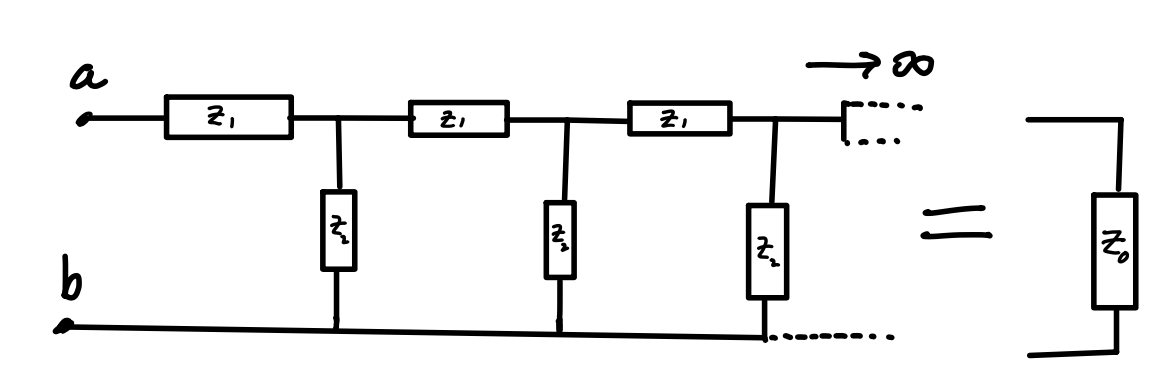
\includegraphics[scale=0.75]{Figs/Feynman/linezs.png}
\caption{A transmission line modeled by series and parallel impedances in an infinite chain.  Its equivalent impedance would be $Z_0$, which could be found by combining each group from right to left using the rules of series and parallel combinations.}
\label{linezs}
\end{figure}

Well if the infinite line has an impedance $Z_0$ and you add on one more circuit unit to the front of it, it'll still have a impedance $Z_0$, for certainly one more circuit unit won't affect the $Z_0$ from an infinite number of units, right?

In Fig.~\ref{add_one}, we'll add a circuit unit (dotted circle) in front of an element $Z_0$ that is the equivalent impedance found from an infinite number of such circuit units.

\begin{figure}[h]
\centering 
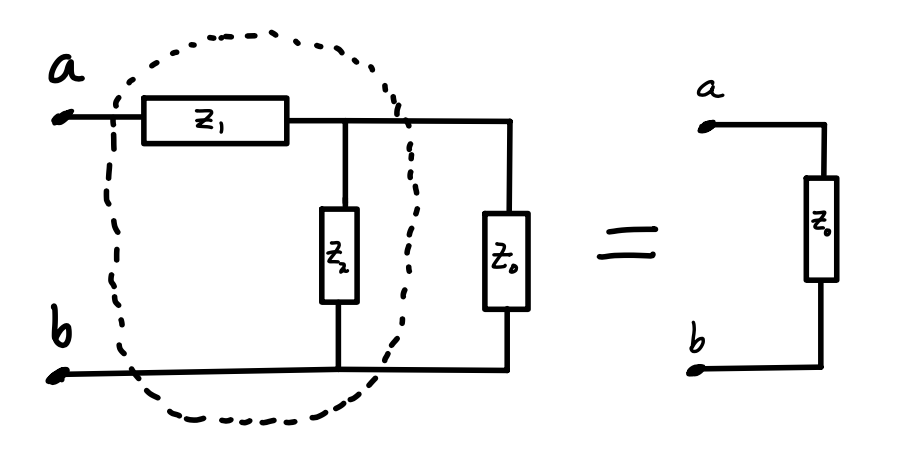
\includegraphics[scale=0.75]{Figs/Feynman/add_one.png}
\caption{Adding one more circuit unit to a $Z_0$ found from an infinite number of units will still result in a total impedance of $Z_0$.}
\label{add_one}
\end{figure}

In this figure, if we find the total impedance like in Fig.~\ref{z04}, we'll get
\begin{equation}
Z_\text{total}=Z_1+\frac{1}{\frac{1}{Z_2}+\frac{1}{Z_0}},
\end{equation}

which shows $Z_2$ and $Z_0$ being combined in parallel, then added to $Z_1$ in series. But remember, adding one unit won't change the fact that's it's all equal to $Z_0$, so we'd get

\begin{equation}
Z_0=Z_1+\frac{1}{\frac{1}{Z_2}+\frac{1}{Z_0}}.
\label{z0_induct}
\end{equation}

This can be solved for $Z_0$ to get
\begin{equation}
Z_0=\frac{Z_1}{2}+\sqrt{\frac{Z_1^2}{4}+Z_1Z_2}.
\label{z0_feyn}
\end{equation}

Now, typically a transmission line is represented by inductors as the series elements and capacitors as the parallel elements as shown in Fig.~\ref{tline}.  Thus, for Eqn.~\ref{z0_feyn}, $Z_1=\omega L$ and $Z_2=1/(\omega C)$. The $\omega L/2$ term in front is a bit inconvenient and may be swept away by claiming that each series inductor has a value of $L/2$ or $L\rightarrow L/2$, giving 

\begin{equation}
Z_0=\sqrt{\frac{L}{C}-\frac{\omega^2L^2}{4}}.
\label{z0_almost}
\end{equation}

\begin{figure}[h]
\centering 
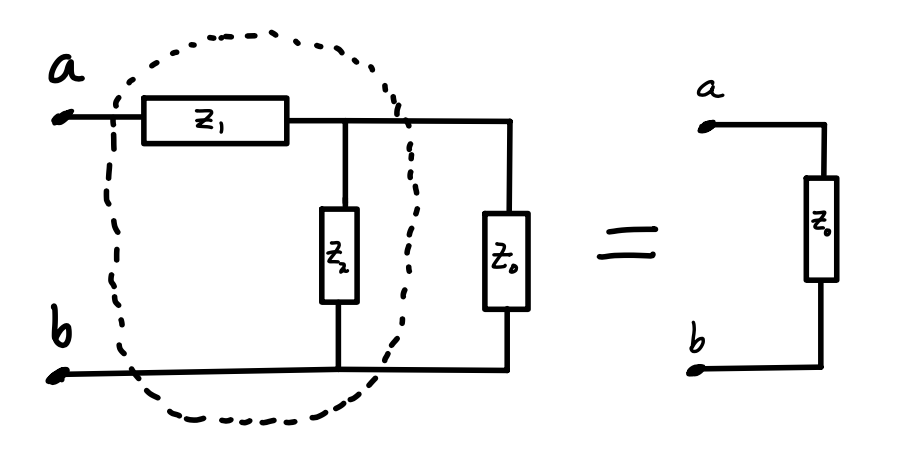
\includegraphics[scale=0.75]{Figs/Feynman/add_one.png}
\caption{A transmission line is represented by an infinite chain of inductors as the series elements and capacitors as the parallel elements.}
\label{tline}
\end{figure}

Now, do a bit of work on Eqn.~\ref{z0_almost}.  In this lab, we used frequencies $<100$ kHz.  If $\omega^2<4/LC$ then it can be dropped from the formula.  Use your best estimates thus far for $L$ and $C$.  Can the term be dropped?  If so, we'll have a comparatively simple expression for the characteristic impedance of the transmission line, $Z_0$, or

\begin{equation}
\label{z0_lc}
Z_0=\sqrt{\frac{L}{C}}.
\end{equation}

\subsection{Evaluate $Z_0$}

Evaluate Eqn.~\ref{z0_lc} in two ways.  First, use your best experimental determinations of $L$ and $C$ to compute $Z$ of the transmission line. 

Second, use your theoretical values for $C$ and $L$ (called ${\tilde C}$ and ${\tilde L}$ above. This should give another formula for $Z_0$, in terms of the geometry of the transmission line or (see Feynman Lecture, Eq. 24.11)

\begin{equation}
Z_0=\frac{\ln(b/a)}{2\pi\epsilon_0 c}.
\end{equation}

Evaluate this equation using the parameters for $b$ and $a$ that you have.  

Note in this equation that $1/(\epsilon_0 c)$ has the dimensions of resistance (Ohms) and is equal to $120\pi$. The $\ln$ dependence on the geometrical parameters is weak, so most coaxial lines have a $Z_0$ in the range of $50$ to a few hundred Ohms (see Feynman, Sect. 24-1).


This is RG-6U coaxial cable, and it's impedance can readily be found online for comparison. At this time, you should have a handful of estimates for $Z_0$. 

\subsection{The far end of the transmission line}

With an expression for the characteristic impedance of a transmission line, let's go back to the oscilloscope display and look at the interesting feature mentioned above. What did you determine it to be? (Hopefully the simulation helped.)

It is a pulse that got {\sl reflected} off of the open-circuited far end of the transmission line, just like you saw in the simulation with the rope. It is not inverted, as in the simulation when a ring is connected to the end and allowed to slide up and down on a pole.  

Anything connected to the far end of the transmission line is called the ``load.'' Loads are electrical, so will have an impedance. Let's call the load $Z_\text{load}$.  In the present case, the load is infinite (nothing is connected to it).  See what happens to the reflection when $Z_\text{load}=0$ (go ahead and connect the two conductors at the far end). The pulse should become inverted, just like in the simulation when the end of the rope was clamped.

What about $Z_\text{load}$ between $0$ and $\infty$?  Let's connect a variable resistor to the end of the transmission line and vary $Z_\text{load}$ and see what happens to the reflection. You can see that the amplitude of the reflected pulse varies with $Z_\text{load}$. As $Z_\text{load}$ is decreased, the amplitude of the reflected pulse decreases as well. The ratio of the reflected pulse amplitude to that of the input pulse amplitude is $\Gamma$, and is called the ``reflection coefficient.'' It is given by

\begin{equation}
\Gamma=\frac{V_\text{reflected}}{V_\text{input}}.
\end{equation}

In terms of the transmission line and load,

\begin{equation}
\label{gamma}
\Gamma=\frac{Z_\text{load}-Z_0}{Z_\text{load}+Z_0}.
\end{equation}

This equation should describe the pulse behavior when $Z_L=\infty$ and $Z_L=0$ (evaluate it at these two values).


\subsection{Data: $\Gamma$ vs $Z_L$}

If we can track $\Gamma$ $(=V_{reflected}/V_{load})$ as a function of $Z_L$ (which we control), we can use Eqn.~\ref{gamma} as another way of finding $Z_0$, the impedance of the transmission line.


Monitor the amplitude of the pulse injected into the transmission line, $V_{input}$. Vary $Z_L$ and record the amplitude of the reflected pulse, $V_{reflected}$.  Plot $\Gamma$ vs $Z_L$. Next do a curve fit to your data with an equation of the form

\begin{equation}
\Gamma=A\frac{Z_L-Z_0}{Z_L+Z_0},
\end{equation}

where the fit parameters are $A$ and $Z_0$, with $A$ being an overall multiplicative constant. We are not quite sure why it $A$ cannot be $1$ to give Eqn.~\ref{gamma}, but allowing it to be a free fit parameter  allows for a pretty close fit to your data. What does the fit give for $Z_0$? Compare your fit $Z_0$ to that from Eqn.~\ref{z0_lc}.

In one more use of Eqn.~\ref{gamma}, what do you think happens to the reflection if $Z_\text{load}=Z_0$, that is, when the load resistance equals the impedance of the cable?  Try this setting and observe the reflected pulse amplitude on the oscilloscope.

When the load on a transmission line equals the impedance of the transmission line, the situation is called ``impedance matching.'' 

\subsection{Derivation: Potential relationship between $Z_\text{load}$ vs. $Z_0$}

In the last section, there was some indication that setting $Z_\text{load}=Z_0$ leads to cancellation of the reflected pulse.  Think now, if there is no reflection, where does all of the initial pulse energy go? (Try to answer this before continuing.)

Suppose we modeled the transmission line and its connected load as two series resistors connected to a voltage source, as shown the figure below.

\begin{figure}[h]
\centering 
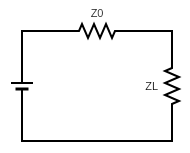
\includegraphics[scale=1]{Figs/circuit.png}
\label{z0zl_circuit}
\end{figure}

Here, $Z_0$ is the transmission line and $Z_\text{load}$ is the load connected to the far end of it.  Compute the power ($P=I^2Z$) flowing through the load. Maximize it with respect to $Z_L$ (i.e. $dP/dZ_\text{load}=0$).  What value of $Z_\text{load}$ will maximize the power delivered to it? 

Once again, this is called ``impedance matching'' and should have some correspondence to what you saw in the previous section. 

To conclude, think about the answer to this question: 

\begin{quote}
``Suppose you are using a transmission line to deliver a signal to some device it is connected to (i.e. the load). To maximize power transmission to the load from the transmission line, the impedance of the load should be \underline{\hspace{1in}}.''
\end{quote}

This is once again called ``impedance matching.'' It is an optimal case when maximum power is delivered from the transmission line to the load.

\section{Wrap-up}

In this lab, you did a pretty thorough experimental and theoretical look at a transmission line.  Your core conclusion would be in your best determination of $Z_0$, the characteristic impedance of the transmission line.  The characteristic impedance silently sat at the core of many of your observations, and indeed drives the overall behavior of a transmission line.


\end{document}
